\documentclass[UTF8]{article}
\usepackage{amsmath, amsthm, amssymb, graphicx, listings, xcolor, geometry, microtype, framed}
\usepackage{CTEX, subfigure}
\usepackage{graphicx}
\geometry{left=2.5cm, right=2.5cm, top=2.5cm, bottom=2.5cm}
\ctexset{today=old}

\title{\textbf{应用数学导论大作业报告}}
\author{陈润璘 2200010848}
\date{\today}

\begin{document}
    \maketitle


    \section{一维有限元方法}

    \subsection{有限元方法}

    \paragraph{(a)}
    我们有:
    \[
        \int_0^L \frac{\textrm{d}u}{\textrm{d}x} \frac{\textrm{d}v}{\textrm{d}x} {\textrm{d}x} =
        -\int_0^L \frac{\textrm{d}^2 u}{\textrm{d}x^2}v {\textrm{d}x}
    \]
    从而
    \[
        \int_0^L \left(\frac{\textrm{d}^2 u}{\textrm{d}x^2} + f\right)v {\textrm{d}x}
    \]
    取
    \[
        v(x)=
        \begin{cases}
            1, & t\le x\le t+\epsilon \\
            0, & else
        \end{cases}
    \]
    其中 $0<t<1$, 有
    \[
        \int_0^L \left(\frac{\textrm{d}^2 u}{\textrm{d}x^2} + f\right)v {\textrm{d}x} = \epsilon \left(\frac{\textrm{d}^2 u}{\textrm{d}x^2} + f\right)(\xi) = 0
    \]
    其中 $t\le\xi\le t + \epsilon$, 令 $\epsilon \to 0$, 有
    \[
        \left(\frac{\textrm{d}^2 u}{\textrm{d}x^2} + f\right)(t) = 0
    \]
    由 $t$ 的任意性,
    \[
        \frac{\textrm{d}^2 u}{\textrm{d}x^2} + f\equiv0,\,\,\forall x\in(0,L)
    \]

    \paragraph{(b)}
    由分部积分:
    \[
        \int_{\Omega}\frac{\textrm{d}(u-u_h)}{\textrm{d}x} \frac{\textrm{d}v_h}{\textrm{d}x}{\textrm d}x =
        (u-u_h)\frac{\textrm{d}v_h}{\textrm{d}x}|_0^L - \int_{\Omega}(u-u_h)\frac{\textrm{d}^2 v_h}{\textrm{d}x^2}{\textrm d}x
    \]
    由于 $(u-u_h)(0) = (u-u_h)(L)=0$ 和 $\frac{\textrm{d}^2 v_h}{\textrm{d}x^2}=0$, 有原式为 0.

    \paragraph{(c)}
    问题 (1.1) 的变分形式为:
    \[
        \int_0^1\frac{\textrm{d}u}{\textrm{d}x} \frac{\textrm{d}v}{\textrm{d}x}{\textrm d}x = \int_0^1 u\textrm{d}x
    \]

    单元个数为 5 时
    \[
        A =
        \begin{pmatrix}
            \frac{1}{h_1}+\frac{1}{h_2} & -\frac{1}{h_2} \\
            -\frac{1}{h_2} & \frac{1}{h_2}+\frac{1}{h_3} & -\frac{1}{h_3} \\
            & -\frac{1}{h_3} & \frac{1}{h_3}+\frac{1}{h_4} & -\frac{1}{h_4}              \\
            &                & -\frac{1}{h_4}              & \frac{1}{h_4}+\frac{1}{h_5} \\
        \end{pmatrix}
    \]

    在这个问题中, 我们取等距的分点, 并使用 Python 来完成计算, 具体代码参见 part2/shared.py 和 part2/problem\_c.py.
    取 $n$ 个分点时, 矩阵 $A$ 的主对角线上的元素为 $2n$, 两条次对角线上的元素为 $-n$, 向量 $b$ 的所有元素都是 $1/n$.

    对于 $n = 10,20,40,80$ 我们使用有限元方法得到的解的图像如下 (图~\ref{fig:figure1}).

    \begin{figure}[h]
        \centering
        \subfigure[$n=10$]{
            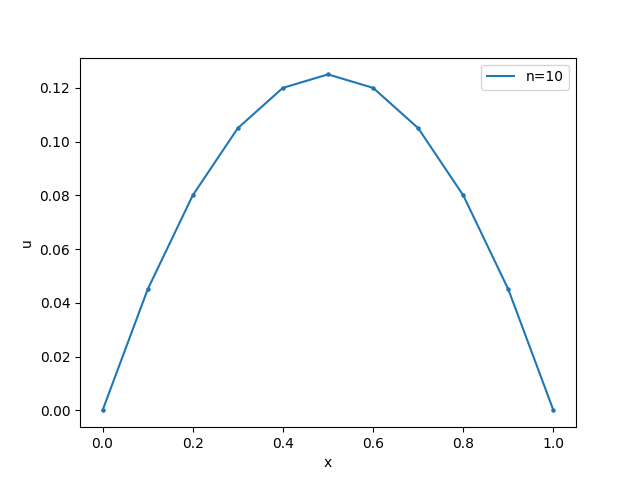
\includegraphics[width=0.45\textwidth]{./assets/10}
        }
        \subfigure[$n=20$]{
            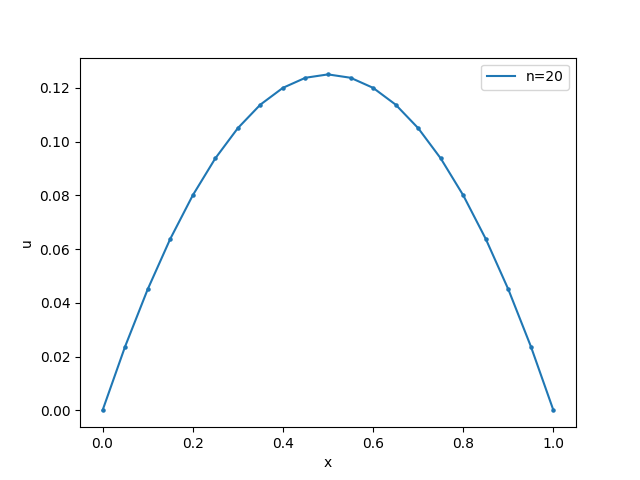
\includegraphics[width=0.45\textwidth]{./assets/20}
        }
        \subfigure[$n=40$]{
            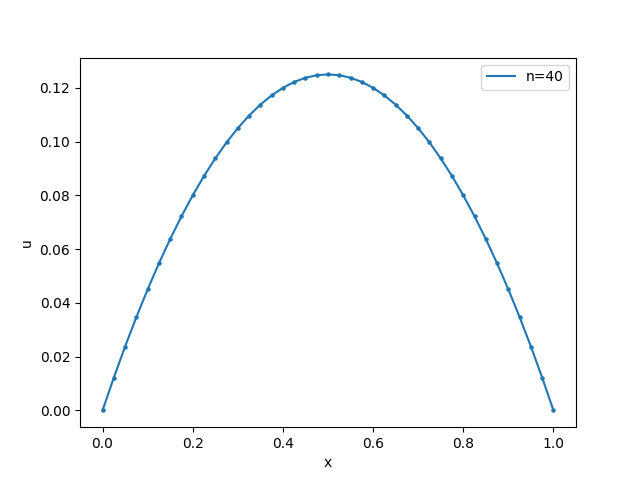
\includegraphics[width=0.45\textwidth]{./assets/40}
        }
        \subfigure[$n=80$]{
            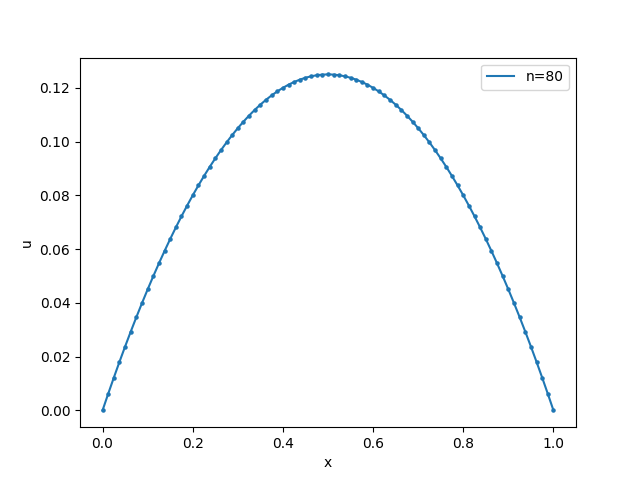
\includegraphics[width=0.45\textwidth]{./assets/80}
        }
        \caption{$n$ 取不同值时解的图像}
        \label{fig:figure1}
    \end{figure}

    从图中可以看出, 随着 $n$ 的增大, 数值解逐渐逼近真实解 $u(x) = x(1-x)$.
    \newline

    \paragraph{(d)}
    对于 $n = 2,4,8,16,32,64.128$, 我们计算了有限元解与真解的误差 $\lVert \frac{\textrm{d}(u-u_h)}{\textrm{d}x} \rVert^2_{L^2(\Omega)}$, 并绘制表格和 log-log 图像 (图~\ref{fig:figure2}, 表~\ref{tab:table1}), 具体代码参见 part2/shared.py 和 part2/problem\_d.py.

    \begin{figure}
        \centering
        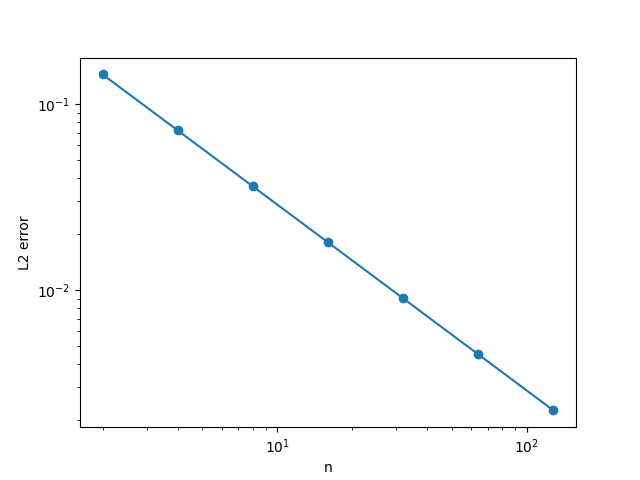
\includegraphics[width=0.4\textwidth]{./assets/fig1}
        \caption{误差随 $n$ 的变化}
        \label{fig:figure2}
    \end{figure}

    \begin{table}
        \centering
        \begin{tabular}{|c|c|}
            \hline
            $n$ & 误差       \\
            \hline
            2   & 0.144338 \\
            4   & 0.072169 \\
            8   & 0.036084 \\
            16  & 0.018042 \\
            32  & 0.009021 \\
            64  & 0.004511 \\
            128 & 0.002255 \\
            \hline
        \end{tabular}
        \caption{误差随 $n$ 的变化}
        \label{tab:table1}
    \end{table}

    从图像和表格中都不难看出,误差大致与 $1/n$ 成正比.

    \subsection{自适应有限元方法}

    在这个问题中,我们求解 $L=1, f=\exp(-100 (x-0.5)^2)$ 的问题.
    由于每一个单元上的误差可以被
    \[
        Ch_i\left( \int_{x_i}^{x_{i+1}} \left( f(x)+ \frac{\textrm{d}^2 u_h}{\textrm{d}x^2}\right)^2 \textrm{d}x \right)^{1/2}
    \]
    控制, 并且在我们的问题中 $u_h$ 时一个分段线性函数, 从而 $\frac{\textrm{d}^2 u_h}{\textrm{d}x^2}$ 是 0, 所以我们可以近似地用
    \[
        h_i\left( \int_{x_i}^{x_{i+1}} f^2(x)\textrm{d}x \right)^{1/2}
    \]
    表示在某个单元上误差的大小, 并在误差较大的单元上加密分点.

    初始时, 我们取十个分点, 并使用有限元方法求解.
    然后我们在每一段上计算 $\eta_j=h_i\left( \int_{x_i}^{x_{i+1}} f^2(x)\textrm{d}x \right)^{1/2}$, 并在每一次迭代时取 $\eta_j>\alpha \max(\eta_i)$ 的单元进行加密, 加密的方法是在原有节点的中点插入一个新的节点, 直到分点数目大于指定值为止.

    我们首先固定 $\alpha=0.5$ 并取 $n<40,80,160$ 进行计算, 得到的解的图像如下~\ref{fig:figure3}.

    \begin{figure}[h]
        \centering
        \subfigure[$n=20$]{
            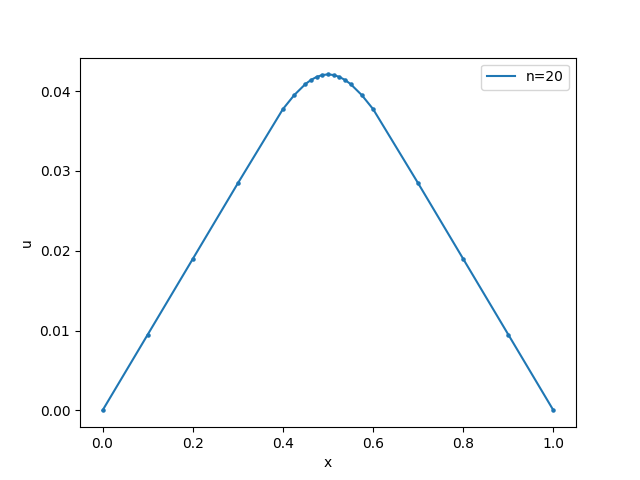
\includegraphics[width=0.4\textwidth]{./assets/adaptive/20}
        }
        \subfigure[$n=40$]{
            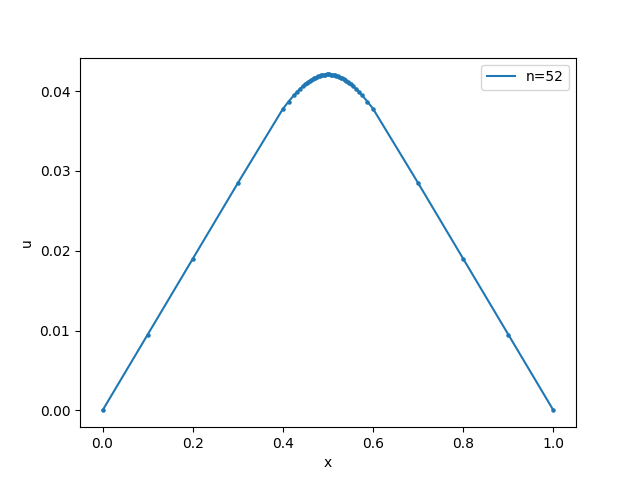
\includegraphics[width=0.4\textwidth]{./assets/adaptive/40}
        }
        \subfigure[$n=80$]{
            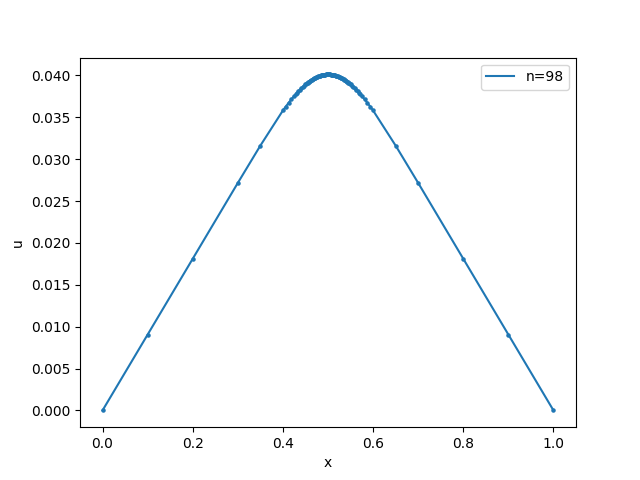
\includegraphics[width=0.4\textwidth]{./assets/adaptive/80}
        }
        \subfigure[$n=160$]{
            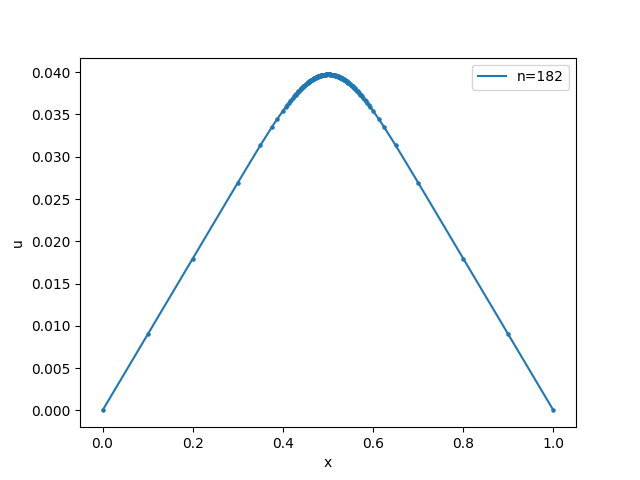
\includegraphics[width=0.4 \textwidth]{./assets/adaptive/160}
        }
        \caption{$n$ 取不同值时解的图像}
        \label{fig:figure3}
    \end{figure}

    从图中可以看出, 随着 $n$ 的增大, 停止迭代时分别取了 52, 98, 182 个分点, 并且新增的分点都集中在函数导数的绝对值较大处, 也就是 $x=0.5$ 附近.
    \newline

    然后,我们固定 $n=80$, 分别取 $\alpha=0.1,0.25,0.5,0.9$ 进行计算, 得到的解的图像如下 (图~\ref{fig:figure4}).

    \begin{figure}[h]
        \centering
        \subfigure[$\alpha=0.1$]{
            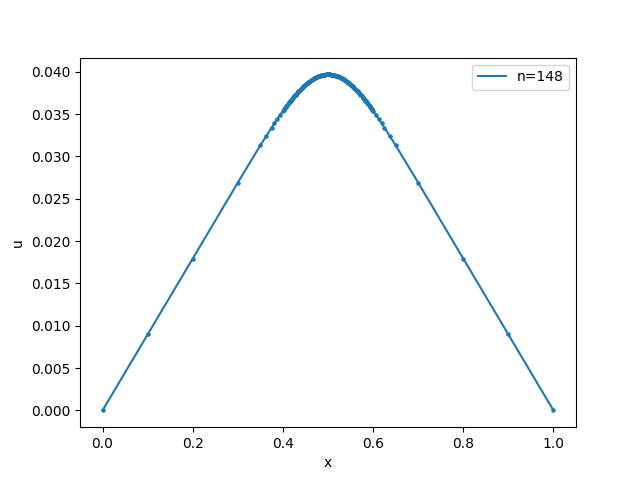
\includegraphics[width=0.4\textwidth]{./assets/adaptive/0_1}
        }
        \subfigure[$\alpha=0.25$]{
            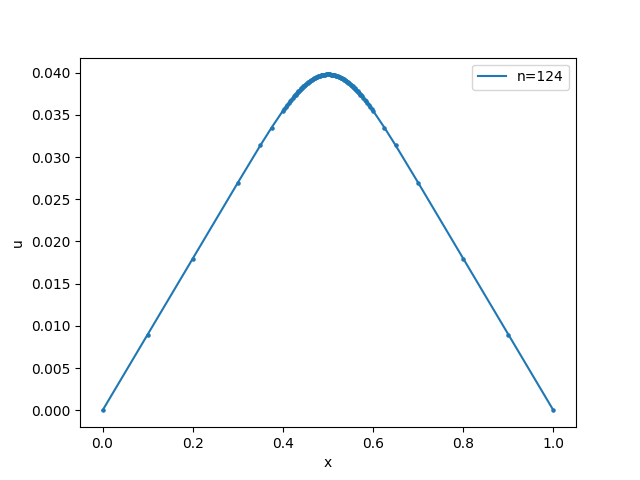
\includegraphics[width=0.4\textwidth]{./assets/adaptive/0_25}
        }
        \subfigure[$\alpha=0.5$]{
            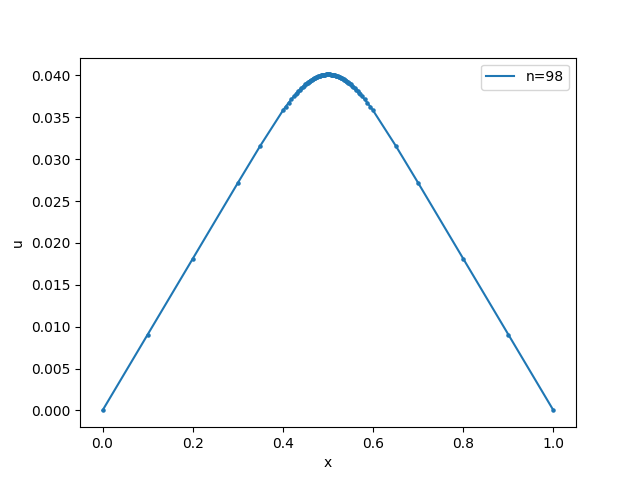
\includegraphics[width=0.4\textwidth]{./assets/adaptive/0_5}
        }
        \subfigure[$\alpha=0.9$]{
            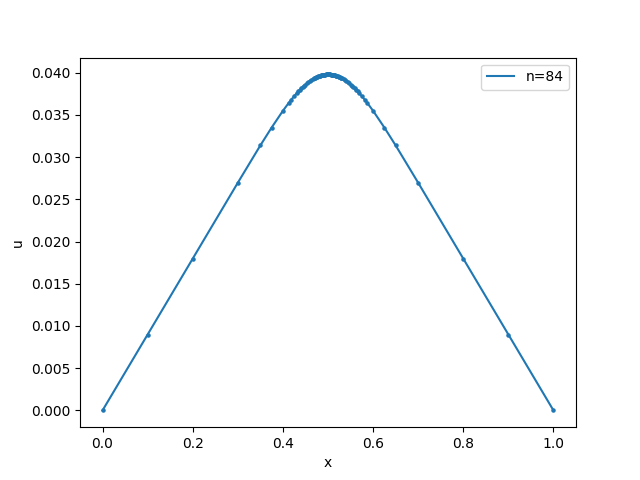
\includegraphics[width=0.4\textwidth]{./assets/adaptive/0_9}
        }
        \caption{$\alpha$ 取不同值时解的图像}
        \label{fig:figure4}
    \end{figure}

    虽然在这四种 $\alpha$ 的取值中, 停止迭代的条件都是相同的, 但是在停止迭代时分别取了 148, 124, 98, 84 个分点, 由此可以看出 $\alpha$ 的取值过小可能会导致过度加密, 从而增加计算量.

    本节的代码参见 part2/adaptive.py.


    \section{二维热传导方程的有限元方法}

    对于二维热传导方程
    \begin{gather*}
        \frac{\partial u(t,x,y)}{\partial t} = \Delta u(t,x,y),\,(x,y)\in\Omega=(0,1)^2,0<t\le 1\\
        u(t,x,y)|_{\partial \Omega} = 0,\,0\le t \le 1\\
        u(0,x,y) = \sin(\pi x)\sin(\pi y)
    \end{gather*}
    我们在空间上使用分片的有限元方法, 在 $\Omega$ 中取均匀的正方形网格, 时间上分别使用显式格式、隐式格式和 Crank-Nicolson 格式进行求解.

    在基函数的选取上, 我们没有选取分片线性基函数, 而是选取了一个二次函数, 它在一个包含 9 个顶点的正方形网格中的中心顶点取 1, 四周的 8 个顶点都取 0.
    更具体地, 它在网格 $(x_0+\delta_1 h,y_0+\delta_2 h),\,\delta_1,\delta_2\in\{-1,0,1\}$ 上的取值为
    \[
        \lambda_{ij}=\frac{(h-| x-x_0 |)(h-| y-y_0 |)}{h^2}
    \]

    我们使用差分近似代替左边对时间的偏导数, 然后在两边同时乘以有上述基函数生成的线性空间中的任何一个函数 $v$, 并在 $\Omega$ 上积分, 有:
    \[
        \int_{\Omega} \frac{u^{n+1}-u^n}{\Delta t}v = -\int_{\Omega} \nabla u\cdot\nabla v
    \]
    对于三种格式, 右边的 $\nabla u$ 可以分别取为 $\nabla u^n, \nabla u^{n+1}, (\nabla u^n+\nabla u^{n+1})/2$.

    以显示格式为例, 设 $u = \Sigma u_{ij}\lambda_{ij}, v = \Sigma v_{ij}\lambda_{ij}$, 代入上式, 有:
    \[
        AU^{n+1} = BU^n
    \]
    其中
    \begin{gather*}
        U^n = \begin{pmatrix}
                  u_{00}^n & u_{01}^n & \cdots & u_{0n}^n & u_{10}^n & \cdots & u_{nn}^n
        \end{pmatrix}^T\\
        A =
        \begin{pmatrix}
            A_1 & A_2    &        &        &     \\
            A_2 & A_1    & A_2    &        &     \\
            & \ddots & \ddots & \ddots &     \\
            &        & A_2    & A_1    & A_2 \\
            &        &        & A_2    & A_1 \\
        \end{pmatrix}\\
        A_1 =
        \begin{pmatrix}
            \frac{4}{9} & \frac{1}{9} & 0           & \cdots & 0           \\
            \frac{1}{9} & \frac{4}{9} & \frac{1}{9} & \cdots & 0           \\
            0           & \frac{1}{9} & \frac{4}{9} & \cdots & 0           \\
            \vdots      & \vdots      & \vdots      & \ddots & \vdots      \\
            0           & 0           & 0           & \cdots & \frac{4}{9} \\
        \end{pmatrix},\,
        A_2 =
        \begin{pmatrix}
            \frac{1}{9}  & \frac{1}{36} & 0            & \cdots & 0           \\
            \frac{1}{36} & \frac{1}{9}  & \frac{1}{36} & \cdots & 0           \\
            0            & \frac{1}{36} & \frac{1}{9}  & \cdots & 0           \\
            \vdots       & \vdots       & \vdots       & \ddots & \vdots      \\
            0            & 0            & 0            & \cdots & \frac{1}{9} \\
        \end{pmatrix}\\
        B =
        \begin{pmatrix}
            B_1 & B_2    &        &        &     \\
            B_2 & B_1    & B_2    &        &     \\
            & \ddots & \ddots & \ddots &     \\
            &        & B_2    & B_1    & B_2 \\
            &        &        & B_2    & B_1 \\
        \end{pmatrix}\\
        B_1 =
        \begin{pmatrix}
            \frac{4}{9}-\frac{8}{3}\lambda & \frac{1}{9}+\frac{1}{3}\lambda & 0                              & \cdots & 0                              \\
            \frac{1}{9}+\frac{1}{3}\lambda & \frac{4}{9}-\frac{8}{3}\lambda & \frac{1}{9}+\frac{1}{3}\lambda & \cdots & 0                              \\
            0                              & \frac{1}{9}+\frac{1}{3}\lambda & \frac{4}{9}-\frac{8}{3}\lambda & \cdots & 0                              \\
            \vdots                         & \vdots                         & \vdots                         & \ddots & \vdots                         \\
            0                              & 0                              & 0                              & \cdots & \frac{4}{9}-\frac{8}{3}\lambda \\
        \end{pmatrix},\,
        B_2 =
        \begin{pmatrix}
            \frac{1}{9}+\frac{1}{3}\lambda  & \frac{1}{36}+\frac{1}{3}\lambda & 0                               & \cdots & 0                              \\
            \frac{1}{36}+\frac{1}{3}\lambda & \frac{1}{9}+\frac{1}{3}\lambda  & \frac{1}{36}+\frac{1}{3}\lambda & \cdots & 0           \\
            0                               & \frac{1}{36}+\frac{1}{3}\lambda & \frac{1}{9}+\frac{1}{3}\lambda  & \cdots & 0                              \\
            \vdots                          & \vdots                          & \vdots                          & \ddots & \vdots                         \\
            0                               & 0                               & 0                               & \cdots & \frac{1}{9}+\frac{1}{3}\lambda \\
        \end{pmatrix}\\
        \lambda = \frac{\Delta t}{h^2}
    \end{gather*}

    使用这种方法得到的线性方程组的阶数很高, 并且系数矩阵是 $n$-对角的对称矩阵, 因此我们可以使用 分块 $LDL^T$ 方法进行求解, 并对存储和计算进行优化.
    由于计算量较大, 为了提升计算的速度, 我们使用 C++ 实现了这个算法.

    在实际计算中, 我们发现隐式格式和 Crank-Nicolson 格式的稳定性均好于显示格式.
    例如, 当空间方向的单元数为 $n^2$ 时, 时间方向上的分点也取 $n^2$ 时, 隐式格式和 Crank-Nicolson 格式都是稳定的, 二显示格式不是稳定的.
    为了使三种格式都是稳定的, 我们取时间方向上的分点个数为 $12n^2$.

    画出三种格式的解的误差关于 $n$ 的图像如下(图~\ref{fig:figure5}, 图~\ref{fig:figure6}).
    从图中可以看出, 无论使用哪一种误差的计算方式, 在数值精度上都是隐式格式 $>$ Crank-Nicolson 格式 $>$ 显式格式.
    我们还可以看出, 三种格式使用 $\|u(1,x,y)-u_h(1,x,y)\|_0$ 计算出的误差都大致与 $1/n^{-2}$ 成正比, 隐式格式使用 $\|\nabla(u(1,x,y)-u_h(1,x,y))\|_0$ 计算出的误差都大致与 $1/n^{-1}$ 成正比.

    \begin{figure}[h]
        \centering
        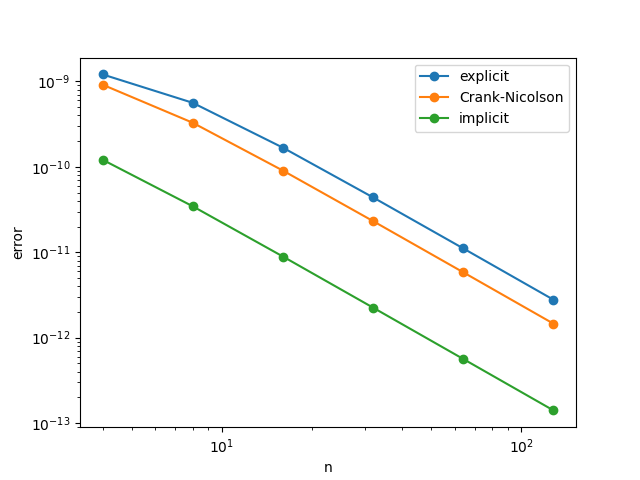
\includegraphics[width=0.7\textwidth]{./assets/L2_error}
        \caption{误差 $\|u(1,x,y)-u_h(1,x,y)\|_0$ 随 $n$ 的变化}
        \label{fig:figure5}
    \end{figure}

    \begin{figure}[h]
        \centering
        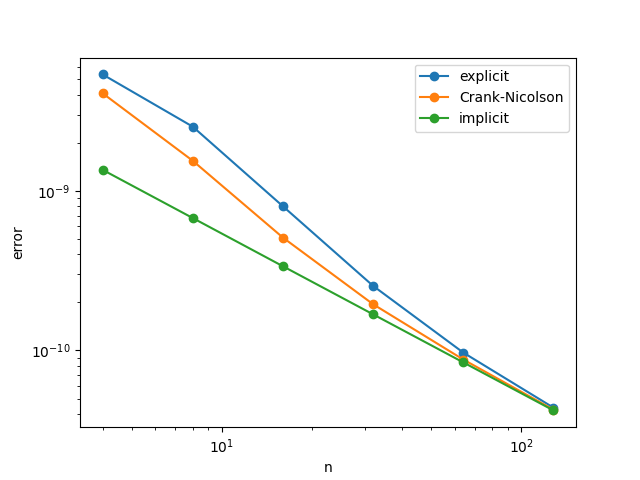
\includegraphics[width=0.7\textwidth]{./assets/H1_error}
        \caption{误差 $\|\nabla(u(1,x,y)-u_h(1,x,y))\|_0$ 随 $n$ 的变化}
        \label{fig:figure6}
    \end{figure}

    本节有限元方法求解的 C++ 代码和编译说明参见 part3/main.cpp, 计算误差的 Python 代码参见 part3/error.py.
\end{document}
